\chapter{Graf przetwarzania sygnałów} \label{dsp_graph_chapter}

Na potrzeby badań zostało zaimplementowane środowisko, pozwalające na dynamiczne tworzenie grafów przetwarzania
sygnałów~(\ref{fig:example_simple_analog_synth}). W projekcie nie zostało zastosowane gotowe rozwiązanie symulujące syntezator modułowy, takie jak
\href{https://www.bespokesynth.com/}{Bespoke Synth}~\cite{bespoke}, \href{https://vcvrack.com/Rack}{VCVRack}~\cite{vcvrack}
lub \href{https://puredata.info/}{Pure Data}~\cite{pure_data}, ponieważ
nie udostępniały one gotowego interfejsu pozwalającego na łatwą integrację z językiem \texttt{Python}.
Istniejące w internecie gotowe przykłady algorytmów syntezy audio pozwoliły na szybkie zaimplementowanie
środowiska eksperymentowego, które posiada szeroki zbiór dostępnych algorytmów DSP oraz w przystępny sposób
interfejsuje się z językiem \texttt{Python}, co umożliwia wykorzystanie gotowych pakietów obliczeniowych z dziedziny przetwarzania sygnałów.

\begin{figure}[H]
    \centering
    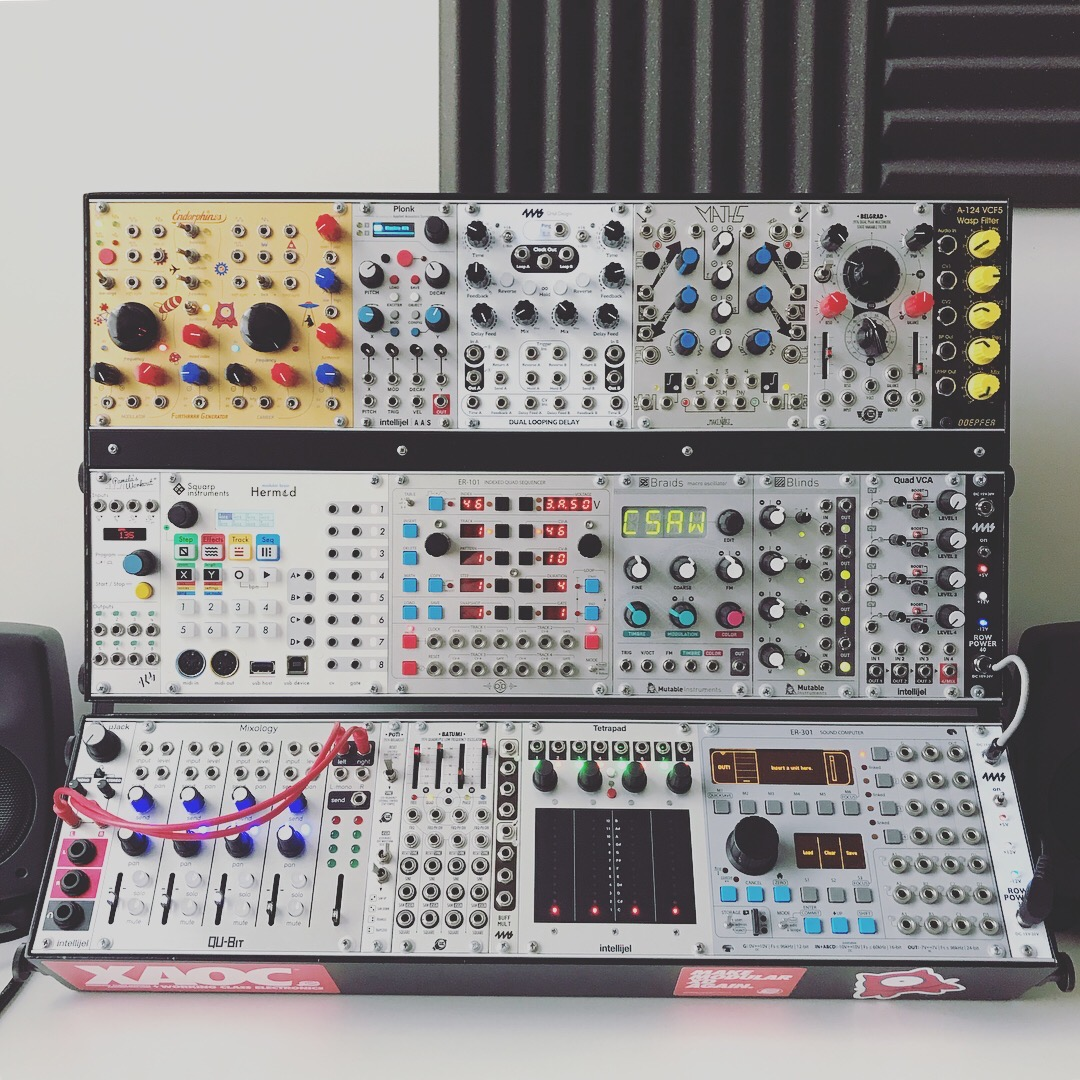
\includegraphics[width=0.4\linewidth]{rys02/eurorack.jpg}
    \caption{
      Przykładowy układ modułów w standardzie \textit{Eurorack}~\cite{eurorack}.
      W prawym dolnym rogu widoczne połączenia modulujące między modułami.
    }
    \label{fig:eurorack_setup}
\end{figure}

\begin{figure}[H]
    \centering
    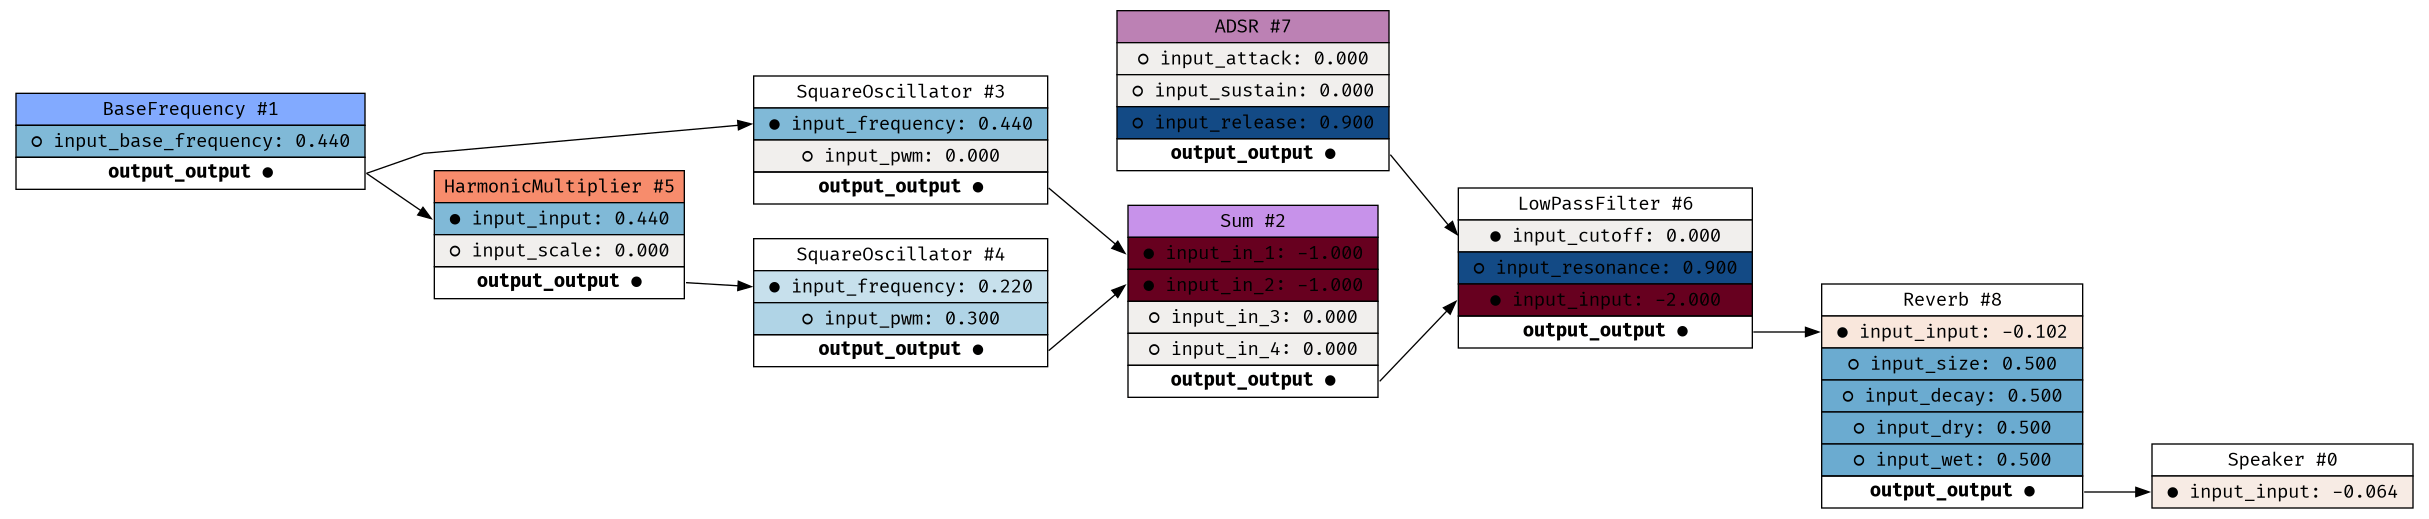
\includegraphics[width=0.9\linewidth]{rys02/luthier_simple_analog.png}
    \caption{
      Przykładowy układ węzłów DSP w zaimplementowanym środowisku eksperymentowym.
      Układ wykonuje syntezę subtraktywną z modulowaną wartością częstotliwości granicznej filtru niskoprzepustowego
      oraz dodaje efekt pogłosu (\textit{reverb})~\cite{reverb}.
    }
    \label{fig:example_simple_analog_synth}
\end{figure}


\section{Podstawy syntezy dźwięku w syntezatorach modułowych}

Proces syntezy dźwięku może zostać przedstawiony jako zbiór węzłów wykonujących syntezę lub
przetwarzanie sygnału audio oraz połączeń między węzłami. Przykładowe elementy grafu:

\begin{enumerate}
  \item Węzły:
    \begin{enumerate}
      \item generujące sygnał:
        \begin{itemize}
          \item synteza sygnałów (sinusoida, trójkąt, sygnał prostokątny),
          \item sygnał modulujący (LFO, ADSR).
        \end{itemize}
      \item przetwarzające sygnał:
        \begin{itemize}
          \item filtry (górnoprzepustowy, dolnoprzepustowy, pasmowo-przepustowy),
          \item efekty (pogłos, echo).
        \end{itemize}
    \end{enumerate}
  \item Połączenia między węzłami:
    \begin{itemize}
      \item modulowanie parametrów syntezy i przetwarzania sygnału.
    \end{itemize}
\end{enumerate}

\noindent
Odpowiednikiem implementowanego środowiska w świecie rzeczywistym są syntezatory modułowe (przykładowo~\ref{fig:eurorack_setup}),
które pozwalają na dowolne łączenie modułów wykonujących operacje DSP.
Barwę dźwięku w syntezatorze modyfikuje się na dwa sposoby:
\begin{enumerate}
  \item Ustawienie stałej wartości danego parametru w węźle DSP,
  \item Modulacja wartości danego parametru w węźle DSP za pomocą wartości wyjściowej innego węzła.
\end{enumerate}

\noindent
Dla przykładowego układu DSP, przedstawionego na rysunku~\ref{fig:example_simple_analog_synth},
skonfigurowane są między innymi parametry:

\begin{enumerate}
  \item Częstotliwość podstawowa (węzeł \texttt{BaseFrequency \#1}),
  \item wartość, przez którą mnożona jest częstotliwość podstawowa w węźle \texttt{HarmonicMultiplier \#5},
  \item Wartości \texttt{input\_pwm} w węzłach \texttt{SquareOscillator} \texttt{\#3} oraz \texttt{\#4},
  \item Parametry algorytmu pogłosu w węźle \texttt{Reverb \#8}.
\end{enumerate}

\noindent
Z kolei wartość parametru \texttt{input\_cutoff} w węźle \texttt{LowPassFilter \#6} modulowana
jest przez sygnał wychodzący w węźle \texttt{ADSR \#7}, co pozwala na dynamiczne zmiany
częstotliwości odcięcia filtru w czasie, wzbogacając barwę generowanego dźwięku.

\section{Wymagania} \label{section:requirements}

W ramach pracy zostały zdefiniowane wymagania dotyczące implementowanego później środowiska eksperymentowego,
opisane w niniejszym rozdziale.

\subsection{Węzły DSP}

Pojedynczy węzeł DSP może zostać opisany za pomocą trzech cech:

\begin{enumerate}
  \item Zbiór sygnałów wejściowych,
  \item zbiór sygnałów wyjściowych,
  \item wykonywana przez węzeł operacja.
\end{enumerate}


% \begin{multicols}{2}
\begin{figure}[H]
    \centering
    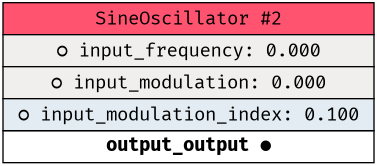
\includegraphics[width=0.4\linewidth]{rys02/example_sine_node.png}
    \caption{
      Węzeł DSP w zaimplementowanym środowisku eksperymentowym, generujący falę sinusoidalną z możliwością modulacji fazy.
    }
    \label{fig:example_sine_node}
\end{figure}

\begin{figure}[H]
    \centering
    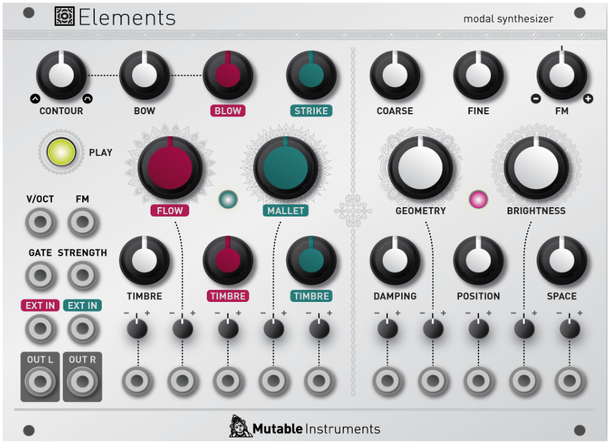
\includegraphics[width=0.45\linewidth]{rys02/mutable_instruments_elements.png}
    \caption{
      Moduł syntezy \textit{Mutable Instruments Elements} umożliwiający modulację
      parametrów syntezy typu \texit{physical modeling}~\cite{lisp_synthesis}.
    }
    \label{fig:example_eurorack_module}
\end{figure}
% \end{multicols}

\noindent
Przykładowo, przedstawiony na rysunku~\ref{fig:example_sine_node} węzeł posiada:
\begin{enumerate}
  \item sygnały wejściowe:
  \begin{itemize}
    \item \texttt{input\_frequency} - częstotliwość generowanej sinusoidy,
    \item \texttt{input\_modulation} - wartość modulacji fazy, według równania~\ref{eq:fm_sine},
    \item \texttt{input\_modulation\_index}.
  \end{itemize}
  \item Sygnały wyjściowe:
  \begin{itemize}
    \item \texttt{output\_output} - wartość generowanego sygnału sinusoidalnego.
  \end{itemize}
\end{enumerate}

\noindent
Węzeł generuje sygnał sinusoidalny o fazie modulowanej poprzez parametr \texttt{input\_modulation} z siłą modulacji ustawianą przez
parametr \texttt{input\_modulation\_index}, opisane za pomocą równania~\ref{eq:fm_sine} oraz listingu~\ref{lst:sine_fm}.

\begin{equation} \label{eq:fm_sine}
  f(t, f, m, m_i) = sin(t * f + m * m_i)
\end{equation}

\begin{lstlisting}[language=Rust, caption=Implementacja węzła SineOscillator.,label={lst:sine_fm}]
impl DspNode for SineOscillator {
    fn tick(&mut self) {
        let frequency = (self.input_frequency * 1000.0).abs();
        let phase_diff = (2.0 * std::f64::consts::PI * frequency) / SAMPLE_RATE;
        self.output_output =
            (self.phase + self.input_modulation * self.input_modulation_index * 10.0).sin();
        self.phase += phase_diff;

        while self.phase > std::f64::consts::PI * 2.0 {
            self.phase -= std::f64::consts::PI * 2.0
        }
    }
}
\end{lstlisting}

\noindent
\textbf{Wymaganie:} zaimplementowane w ramach pracy środowisko eksperymentalne musi pozwalać na zdefiniowanie węzłów DSP, które generują lub
przetwarzają sygnał. Węzły posiadają sloty wejściowe, z których czytają wartości parametrów sterujących wykonywanymi 
przez węzły operacjami.

\subsection{Połączenia między węzłami -- modulacja parametrów węzłów}

Każdy węzeł DSP w środowisku eksperymentowym posiada zbiór parametrów wejściowych. Poza możliwością
ustawienia danego parametru wejściowego na konkretną wartość, możliwa jest też modulacja parametru
wejściowego. Na rysunku~\ref{fig:fm_mod_example} przedstawiony jest przykładowy układ węzłów i modulacji,
które pozwalają na uzyskanie syntezy FM.

\begin{figure}[H]
    \centering
    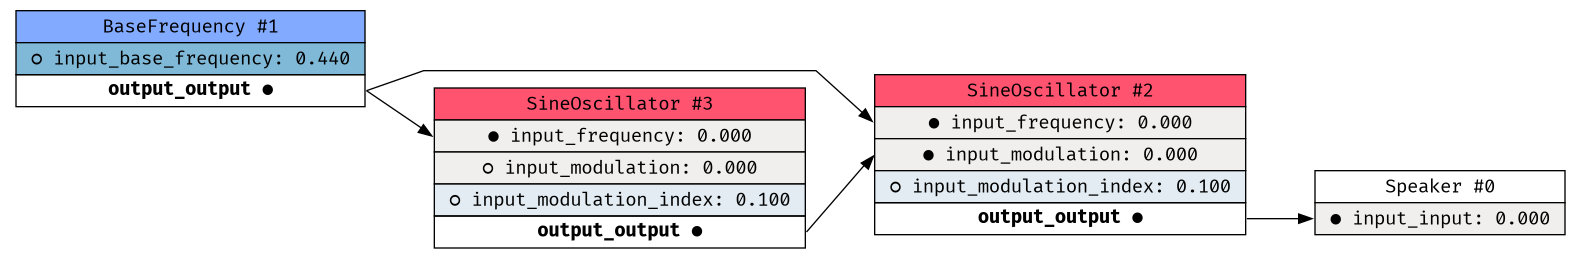
\includegraphics[width=1.0\linewidth]{rys02/fm_mod_example.png}
    \caption{
      Przykładowa modulacja parametru \texttt{input\_modulation} za pomocy sygnału sinusoidalnego, charakterystyczna dla syntezy typu FM \cite{computational_music_synthesis}.
    }
    \label{fig:fm_mod_example}
\end{figure}

\begin{multicols}{2}
\begin{figure}[H]
    \centering
    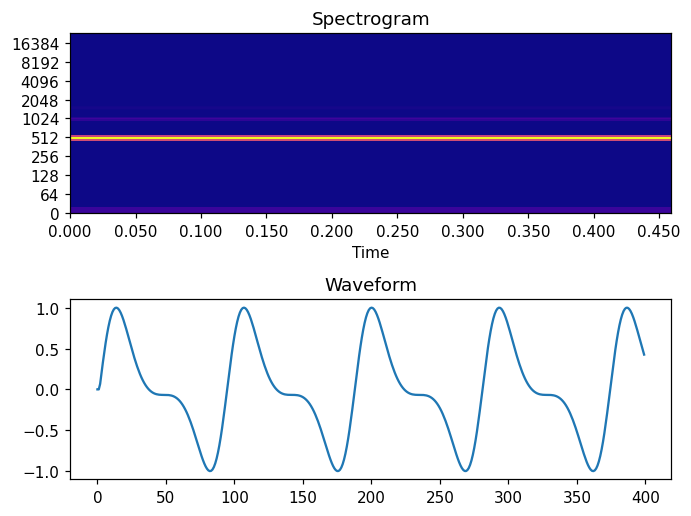
\includegraphics[width=1.0\linewidth]{rys02/spectro_fm.png}
    \caption{
      Spektrogram oraz wykres sygnału wygenerowanego za pomocą układ z rysunku~\ref{fig:fm_mod_example}.
      Widoczne dodatkowe składowe harmoniczne wpływające na barwę dźwięku.
    }
    \label{fig:fm_mod_spectra}
\end{figure}

\begin{figure}[H]
    \centering
    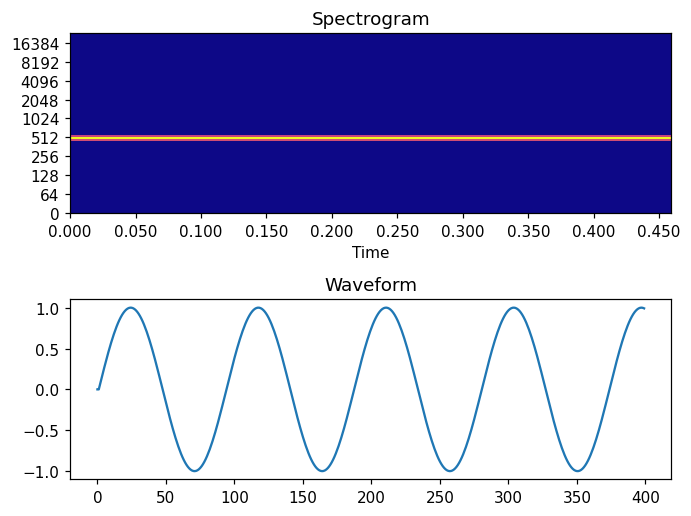
\includegraphics[width=1.0\linewidth]{rys02/spectro_no_fm.png}
    \caption{
      Spektrogram oraz wykres sygnału wygenerowanego przez układ z rysunku~\ref{fig:fm_mod_example}
      \textbf{po usunięciu} połączenia modulującego fazę oscylatora \texttt{\#2}.
      Widoczna tylko jedna składowa harmoniczna: częstotliwość podstawowa.
    }
    \label{fig:fm_no_mod_spectra}
\end{figure}
\end{multicols}

\noindent
\textbf{Wymaganie:} zaimplementowane środowisko pozwala na modulowanie
dowolnego parametu wejściowego w węźle za pomocą wartości wyjściowej dowolnego węzła,
\textbf{w tym modulowanie wejścia węzła wyjściem tego samego węzła} (tzw. \textit{circular patching},
popularny zarówno w syntezie FM jak i w układach analogowych).

\subsection{Graf przetwarzania sygnałów}

Węzły DSP oraz połączenia między nimi istnieją w ramach danego grafu przetwarzania sygnałów, który agreguje
wiele węzłów i wiele połączeń. Instancja grafu DSP musi umożliwiać dynamiczną modyfikację grafu, na którą składają się następujące operacje:

\begin{enumerate}
  \item Dodanie nowego węzła,
  \item Dodanie nowego połączenia między węzłami,
  \item Usunięcie węzła,
  \item Usunięcie połączenia między węzłami,
  \item Ustawienie $i$-tego parametru wejściowego danego węzła na określoną przez użytkownika wartość.
\end{enumerate}

\noindent
Po utworzeniu grafu, użytkownik musi mieć możliwość ,,uruchomienia'' na grafie procesu syntezy dźwięku,
który zwróci użytkownikowi strukturę danych zawierającą wygenerowany sygnał. \\

\noindent
\textbf{Wymaganie:} zaimplementowane środowisko pozwala na dynamiczną modyfikację grafu przetwarzania sygnałów oraz na 
wygenerowanie sygnału z wytworzonego w środowisku grafu.


\subsection{Automatyzacja pracy ze środowiskiem eksperymentowym za pośrednictwem języka \texttt{Python}}

\textbf{Wymaganie:} ze względu na dużą dostępność gotowych algorytmów optymalizacyjnych oraz DSP w języku \texttt{Python}
(\cite{librosa}, \cite{2020SciPy-NMeth}), zaimplementowane środowisko musi udostępniać interfejs pozwalający
na wykonywanie operacji zdefiniowanych w wymaganiach za pośrednictwem języka \texttt{Python}.

\section{Opis zaimplementowanego środowiska eksperymentowego}

W ramach pracy zaimplementowane zostało środowisko pozwalające na dynamiczne budowanie grafów DSP oraz
na generowanie sygnałów dźwiękowych za pomocą wytworzonych grafów,
według wymagań opisanych w sekcji~\ref{section:requirements}. Środowisko zaimplementowano w języku \texttt{Rust},
dzięki czemu proces syntezy sygnałów jest szybszy niż w przypadku implementacji w języku interpretowanym.
Zaimplementowana biblioteka udostępnia interfejs zgodny ze standardem
\textit{Python Extension Module}~\cite{python_extension_module}.

\subsection{Przykłady użycia}

Zaimplementowane środowisko pozwala na tworzenie grafów przetwarzania sygnałów za pomocą poleceń w języku \texttt{Python}.
Listing~\ref{lst:simple_sine} przedstawia proces tworzenia prostego grafu generującego sygnał sinusoidalny.

\begin{lstlisting}[language=python, caption=Utworzenie prostego grafu generującego sygnał sinusoidalny., label={lst:simple_sine}]
g = DspGraph()

carrier = g.add_sine(SineOscillator())
g.patch(
  g.base_frequency_node_id, "output_output",
  carrier, "input_frequency"
)

g.patch(
  carrier, "output_output",
  g.speaker_node_id, "input_input"
)

display(Image(g.draw()))
\end{lstlisting}

\begin{figure}[H]
    \centering
    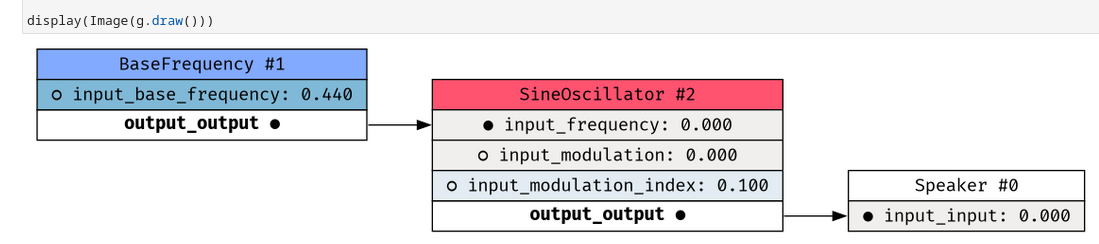
\includegraphics[width=1.0\linewidth]{rys02/simple_graph_creation_example.png}
    \caption{
      Wynik wykonania kodu przedstawionego w listingu~\ref{lst:simple_sine} w środowisku \textit{Jupyter Notebook},
      wizualizacja utworzonego grafu.
    }
    \label{fig:example_graph_creation_jupyter}
\end{figure}


Jak pokazano na listingu~\ref{lst:numpy_rust}, środowisko eksperymentalne zaimplementowane w ramach pracy w języku \texttt{Rust}
zwraca obiekty typu \texttt{ndarray}, wykorzystywane w większości pakietów obliczeniowych wykorzystywanych w języku \texttt{Python}.
Umożliwia to wykorzystanie gotowych bibliotek dostępnych w języku \texttt{Python},
aby przeanalizować sygnał lub zoptymalizować parametry syntezy \cite{2020SciPy-NMeth} \cite{librosa}.


\begin{lstlisting}[language=python, caption=Typ danych zwracanych przez środowisko eksperymentalne., label={lst:numpy_rust}]
>>> generated_signal = g.play(num_samples=100)
>>> type(generated_signal)
<class `numpy.ndarray'>
\end{lstlisting}

% \cite{computational_music_synthesis}

% Szablon powinien dać się skompilować w dowolnym środowisku, w którym zainstalowano system \LaTeX. 
% Zalecaną konfiguracją, która działa w systemie Windows, jest: \texttt{MiKTeX} (windowsowa dystrybucja latexa) + \texttt{TeXnicCenter} (środowisko do edycji i kompilacji projektów latexowych) + \texttt{SumatraPDF} (przeglądarka pdfów z nawigacją zwrotną) + \texttt{JabRef} (opcjonalny edytor bazy danych bibliograficznych). Narzędzia te można pobrać ze stron internetowych, których adresy zamieszczono w tabeli~\ref{tab:narzedzia}. 
% \begin{table}[htb] \small
% \centering
% \caption{Wykaz zalecanych narzędzi do pracy z wykorzystaniem szablonu (na dzień 09.02.2021)}
% \label{tab:narzedzia}
% \begin{tabularx}{\linewidth}{|c|c|X|p{5.5cm}|} \hline\
% Narzędzie & Wersja & Opis & Adres \\ \hline\hline
% \texttt{MiKTeX} & 22.12 & Zalecana jest instalacja \texttt{Basic MiKTeX} 32 lub 64 bitowa. Brakujące pakiety będą się doinstalowywać podczas kompilacji projektu &
% \url{http://miktex.org/download} \\ \hline
% \texttt{TeXnicCenter} & 2.02 &  Można pobrać 32 lub 64 bitową wersję & \url{http://www.texniccenter.org/download/} \\ \hline
% \texttt{SumatraPDF} & 3.4.6 & Można pobrać 32 lub 64 bitową wersję & \url{http://www.sumatrapdfreader.org/download-free-pdf-viewer.html} \\ \hline
% \texttt{JabRef} & 5.7	 & Rozwijane w JDK 15, ma własny instalator i wersję przenośną & \url{http://www.fosshub.com/JabRef.html} \\ \hline
% \end{tabularx}
% \end{table}

% Wspomniana nawigacja między \texttt{TeXnicCenter} a \texttt{SumatraPDF} polega na przełączaniu się pomiędzy tymi narzędziami z zachowaniem kontekstu położenia kursora. Czyli edytując tekst w \texttt{TeXnicCenter} po kliku na ikonce podglądu można przeskoczyć do odpowiedniego miejsca w pdfie wyświetlanym przez \texttt{SumatraPDF}. Podwójne kliknięcie zaś w pdfie widocznym w \texttt{SumatraPDF} ustawi kursor we właściwym akapicie w edytorze tekstu \texttt{TeXnicCenter}. O konfiguracji obu narzędzi do takiej współpracy napisano na stronie \url{http://tex.stackexchange.com/questions/116981/how-to-configure-texniccenter-2-0-with-sumatra-2013-2014-2015-version} (w sieci można znaleźć również inne materiały na ten temat).

% Szablon można również kompilować za pomocą innych narzędzi i środowisk (np.\ za pomocą multiplatformowego \texttt{TexStudio} oraz różnych dystrybucji systemu \LaTeX). Może to jednak czasem wymagać zmiany sposobu kodowania plików i korekty deklaracji kodowania znaków w dokumencie głównym (co opisano dalej). 
% Można go też zaadoptować do wymogów \LaTeX-owych edytorów i kompilatorów działających w trybie on-line, oferowanych na przykład w usłudze \texttt{Overleaf} (\url{https://www.overleaf.com/}). 

% Choć usługa \texttt{Overleaf} ma niewątpliwie wiele zalet (pozwala na edycję kodu przez wielu użytkowników jednocześnie), to podczas pracy nad długimi dokumentami przegrywa ona ze wspomnianymi zintegrowanymi środowiskami \texttt{TeXnicCenter} czy \texttt{TexStudio}. W \texttt{Overleaf} nie można wyświetlić struktury całego projektu (a jedynie listę plików projektowych oraz strukturę bieżąco edytowanego dokumentu), nie można uruchomić wyszukiwania we wszystkich plikach projektowych (nie ma opcji  \texttt{Find in Files...}, która bardzo się przydaje, gdy nie wiadomo, w~którym pliku jest wyszukiwany tekst). 


% \texttt{Overleaf} wymaga użycia kodowania UTF8. Czyli aby dało się wczytać niniejszy szablon pracy dyplomowej do tego środowiska, pliki szablonu muszą być przekodowane, muszą też być zmienione opcje pakietu \texttt{inputenc} oraz odpowiednio zadeklarowane \texttt{literate} (aby dało się używać polskich znaków na listingach). Aby sprawę uprościć przygotowano dwie wersje szablonu: w kodowaniu ANSI oraz UTF8.

% Choć w \texttt{Overleaf} istnieje możliwość skorzystania z wersjonowania (system ten integruje się z repozytorium \texttt{git}), to wersjonowanie to nie działa perfekcyjnie. Dlatego \textbf{zaleca się korzystanie ze środowisk zintegrowanych zainstalowanych lokalnie, czemu towarzyszyć ma wersjonowanie z pomocą wybranego zdalnego repozytorium (\texttt{gitlab}, \texttt{github}, \texttt{bitbucket})}.

% \section{Struktura projektu}
% Pisząc pracę w systemie \LaTeX zwykle przyjmuje się jakąś konwencję co do nazewnictwa tworzonych plików, ich położenia oraz powiązań. Przygotowując niniejszy szablon założono, że projekt będzie się składał z pliku głównego, plików z kodem kolejnych rozdziałów i dodatków (włączanych do kompilacji w dokumencie głównym), katalogów z plikami grafik (o nazwach wskazujących na rozdziały, w których grafiki te zostaną wstawione), pliku ze skrótami (opcjonalny), pliku z danymi bibliograficznymi (plik \texttt{dokumentacja.bib}). Taki ,,układ'' zapewnia porządek oraz pozwala na selektywną kompilację rozdziałów. 

% Przyjętą konwencję da się opisać jak następuje:
% \begin{itemize}
% \item Plikiem głównym jest plik \texttt{Dyplom.tex}. To w nim znajdują się deklaracje wszystkich używanych styli, definicje makr oraz ustawień, jak również polecenie \verb+\begin{document}+. W~nim też należy ustawić metadane, które pojawią się na stronie tytułowej (oraz w stopkach).
% \item Teksty redagowane są w osobnych plikach. Pliki te zamieszczone są w katalogu głównym (tym samym, co plik \texttt{Dyplom.tex}).
% \item W pliku \texttt{streszczenie.tex} powinien pojawić się tekst streszczenia ze słowami kluczowymi (tekst ten oraz słowa kluczowe będzie można wykorzystać do wypełnienia formularzy pojawiających się podczas wysyłania pracy do analizy antyplagiatowej w systemie ASAP)
% \item Plik \texttt{skroty.tex} powinien zawierać wykaz użytych skrótów. Można z tego pliku zrezygnować, jeśli liczba stosowanych skrótów jest nieznaczna. 
% \item Tekst kolejnych rozdziałów powinien pojawić się w plikach o nazwach zawierających numery tych rozdziałów. Według przyjętej konwencji \texttt{rozdzial01.tex} to plik pierwszego rozdziału, \texttt{rozdzial02.tex} to plik z treścią drugiego rozdziału itd. 
% \item Teksty dodatków mają być zapisywane w osobnych plikach o nazwach zawierających literę dodatku. Pliki te, podobnie do plików z tekstem rozdziałów, zamieszczane są w katalogu głównym. I~tak \texttt{dodatekA.tex} oraz \texttt{dodatekB.tex} to, odpowiednio, pliki z treścią dodatku A oraz dodatku B.
% \item Każdemu rozdziałowi i dodatkowi towarzyszy katalog przeznaczony do składowania dołączanych grafik. I tak \texttt{rys01} to katalog na pliki z grafikami dołączanymi do rozdziału pierwszego, \texttt{rys02} to katalog na pliki z grafikami dołączanymi do rozdziału drugiego itd.
% Podobnie \texttt{rysA} to katalog na pliki z grafikami dołączanymi w dodatku A itd.
% \item W katalogu głównym zamieszczany jest plik \texttt{dokumentacja.bib} zawierający bazę danych bibliograficznych.
% \item Jeśli praca nad dokumentem odbywa się w \texttt{TeXnicCenter}, to zgodnie z wymogami tego narzędzia powinien istnieć jeszcze dodatkowy plik projektu. Plik ten pełni podobną rolę jak plik solucji wykorzystywany w zintegrowanych środowiskach programowania. Co prawda plik projektu nie jest wymagany do \LaTeX-owej kompilacji (wystarczy kompilować plik główny), niemniej pozwala zapamiętać ustawienia środowiska (w tym ustawienia językowe potrzebne do sprawdzania poprawności wyrazów -- patrz następny podrozdział).  Plik projektu dostarczony w szablonie ma nazwę \texttt{Dyplom.tcp}. 
% \end{itemize}

% \begin{table}[htb]
% \centering\small
% \caption{Pliki źródłowe szablonu oraz wyniki kompilacji}
% \label{tab:szablon}
% \begin{tabularx}{\linewidth}{|p{.55\linewidth}|X|}\hline
% Źródła & Wyniki kompilacji \\ \hline\hline
% \verb?Dokument.tex? - dokument główny\newline
% \verb?Dokument.tcp? -- plik projektu \verb+TeXnicCenter+\newline
% \verb?streszczenie.tex? -- plik streszczenia\newline
% \verb?skroty.tex? -- plik ze skrótami\newline
% \verb?rozdzial01.tex? -- plik rozdziału \texttt{01}\newline
% \verb?...?\newline
% \verb?dodatekA.tex? -- plik dodatku \texttt{A}\newline
% \verb?...?\newline
% \verb?rys01? -- katalog na rysunki do rozdziału \texttt{01}\newline
% \verb?   |- fig01.png? -- plik grafiki\newline
% \verb?   |- ...?\newline
% \verb?...?\newline
% \verb?rysA? -- katalog na rysunki do dodatku \texttt{A}\newline
% \verb?   |- fig01.png? -- plik grafiki\newline
% \verb?   |- ...?\newline
% \verb?...?\newline
% \verb?dokumentacja.bib? -- plik danych bibliograficznych\newline
% \verb?Dyplom.ist? -- plik ze stylem indeksu\newline
% \verb?by-nc-sa.png? -- plik z ikonami CC\newline
%  &
% \verb?Dyplom.bbl?\newline
% \verb?Dyplom.blg?\newline
% \verb?Dyplom.ind?\newline
% \verb?Dyplom.idx?\newline
% \verb?Dyplom.lof?\newline
% \verb?Dyplom.log?\newline
% \verb?Dyplom.lot?\newline
% \verb?Dyplom.out?\newline
% \verb?Dyplom.pdf? -- dokument wynikowy\newline
% \verb?Dyplom.syntex?\newline
% \verb?Dyplom.toc?\newline
% \verb?Dyplom.tps?\newline
% \verb?*.aux?\newline 
% \verb?Dyplom.synctex?\newline\\
% \hline
% \end{tabularx}
% \end{table}

% \section{Kodowanie znaków}
% System \LaTeX obsługuje wielojęzyczność. Można tworzyć w nim dokumenty z tekstem zawierającym różne znaki diakrytyczne. 
% Należy jednak zdawać sobie sprawę, w jaki sposób znaki te są obsługiwane. Na kodowanie znaków należy patrzeć z dwóch perspektyw: perspektywy edytowania kodu źródłowego oraz perspektywy kodowania dokumentu wynikowego i użytych czcionek.

% Kod latexowy może być edytowany w dowolnym edytorze tekstów. Zastosowane kodowanie znaków w tym edytorze musi być znane \LaTeX-owi, inaczej kompilacja tego kodu się nie powiedzie. Informację o tym kodowaniu przekazuje się w opcjach pakietu \texttt{inputenc}. Niniejszy szablon przygotowano w systemie Windows, a \LaTeX-owe źródła umieszczono w plikach ANSI z użyciem strony kodowej cp1250. Dlatego w poleceniu \verb+\usepackage[cp1250]{inputenc}+ jako opcję wpisano \texttt{cp1250}.


% Szablon można wykorzystać również przy innych kodowaniach i w innych systemach. Jednak wtedy konieczna będzie korekta dokumentu \texttt{Dyplom.tex} odpowiednio do wybranego przypadku. Korekta ta polegać ma na zamianie polecenia \verb+\usepackage[cp1250]{inputenc}+  na polecenie \verb+\usepackage[utf8]{inputenc}+ oraz konwersji znaków i zmiany kodowania istniejących plików ze źródłem latexowego kodu (plików o rozszerzeniu \texttt{*.tex} oraz \texttt{*.bib}).

% Kodowanie znaków jest istotne również przy edytowaniu bazy danych bibliograficznych (pliku \texttt{dokumentacja.bib}). Aby \texttt{bibtex} poprawnie interpretował polskie znaki plik \texttt{dokumentacja.bib} powinien być zakodowany w ANSI, CR+LF (dla ustawień jak w szablonie). 
% W szczególności, jeśli ominąć chce się problem kodowania, polskie znaki w bazie danych bibliograficznych można zastąpić odpowiednią notacją: \verb|\k{a}| \verb|\'c| \verb|\k{e}| \verb|\l{}| \verb|\'n| \verb|\'o| \verb|\'s| \verb|\'z| \verb|\.z| \verb|\k{A}| \verb|\'C| \verb|\k{E}| \verb|\L{}| \verb|\'N| \verb|\'O| \verb|\'S| \verb|\'Z| \verb|\.Z|. 

% Samo kodowanie plików może być źródłem paru problemów. Chodzi o to, że użytkownicy pracujący z edytorami tekstów pod linuxem mogą generować pliki zakodowane w UTF8 bez BOM (lub z BOM -- co nie jest zalecane), a pod windowsem -- pliki ANSI ze znakami ze strony kodewej \texttt{cp1250}. Z takimi plikami różne edytory różnie sobie radzą. W szczególności edytor \texttt{TeXnicCenter} podczas otwierania plików może potraktować jego zawartość jako UTF8 lub ANSI -- prawdopodobnie interpretuje z jakim kodowaniem ma do czynienia na podstawie obecności w pliku znaków specjalnych. Bywa, że choć wszystko w \texttt{TeXnicCenter} wygląda na poprawne, to jednak kompilacja \LaTeX-owa ,,nie idzie''. Problemem mogą być właśnie pierwsze bajty, których nie widać w edytorze. 

% Do konwersji kodowania można użyć edytor \texttt{Notepad++} (jest tam opcja ,,konwertuj'' -- nie mylić z~opcją ,,koduj'', która przekodowuje znaki, jednak nie zmienia sposobu kodowania pliku).

% Jeśli chodzi o drugą perspektywę, tj.\ kodowanie znaków w dokumencie wynikowym, to sprawa jest bardziej skomplikowana. Wiąże się z nią zarządzanie czcionkami, definiowanie mapowania itp. 
% \textbf{Szablon przygotowano tak, by wynikowy dokument zawierał polskie znaki diakrytyczne, które nie są zlepkami literki i ogonka.}

% \section{Kompilacja szablonu}
% Kompilację szablonu można uruchamiać na kilka różnych sposobów. Wszystko zależy od używanego systemu operacyjnego, zainstalowanej na nim dystrybucji \LaTeX-a oraz dostępnych narzędzi. Zazwyczaj kompilację rozpoczyna się wydając polecenie z linii komend lub uruchamia się ją za pomocą narzędzi zintegrowanych środowisk.

% Kompilacja z linii komend polega na uruchomieniu w katalogu, w którym rozpakowano źródła szablonu, następującego polecenia:
% \begin{lstlisting}[basicstyle=\ttfamily]
% > pdflatex Dyplom.tex
% \end{lstlisting}
% gdzie \texttt{pdflatex} to nazwa kompilatora, zaś \texttt{Dyplom.tex} to nazwa głównego pliku redagowanej pracy. 
% W przypadku korzystania ze środowiska \texttt{TeXnicCenter} należy otworzyć dostarczony w~szablonie plik projektu \texttt{Dyplom.tcp}, a następnie uruchomić kompilację narzędziami dostępnymi w pasku narzędziowym.

% Aby poprawnie wygenerowały się wszystkie referencje (spis treści, odwołania do tabel, rysunków, pozycji literaturowych, równań itd.) kompilację \texttt{pdflatex} należy wykonać dwukrotnie, a~czasem nawet trzykrotnie. Wynika to z konieczności zapamiętywania pośrednich wyników kompilacji i ich wykorzystywania w kolejnych przebiegach. Tak dzieje się przy generowaniu odwołań do pozycji literaturowych oraz tworzeniu ich wykazu). 

% Wygenerowanie danych bibliograficznych zapewnia kompilacja \texttt{bibtex} uruchamiana po kompilacji \texttt{pdfltex}. Można to zrobić z linii komend:
% \begin{lstlisting}[basicstyle=\ttfamily]
% > bibtex Dyplom
% \end{lstlisting}
% lub wybierając odpowiednią pozycję z paska narzędziowego wykorzystywanego środowiska. Po kompilacji za pomocą \texttt{bibtex} na dysku pojawi się plik \texttt{Dyplom.bbl}. Dopiero po kolejnych dwóch kompilacjach \texttt{pdflatex} dane z tego pliku zostaną odpowiednio przetworzone i zrenderowane w wygenerowanym dokumencie. Tak więc po każdym wstawieniu nowego cytowania w kodzie dokumentu uzyskanie poprawnego formatowania dokumentu wynikowego wymaga powtórzenia następującej sekwencji kroków kompilacji:
% \begin{lstlisting}[basicstyle=\ttfamily]
% > pdflatex Document.tex
% > bibtex Document
% > latex Document.tex
% > latex Document.tex
% \end{lstlisting}
% Szczegóły dotyczące przygotowania danych bibliograficznych oraz zastosowania cytowań przedstawiono w podrozdziale \ref{sec:literatura}.

% W głównym pliku zamieszczono polecenia pozwalające sterować procesem kompilacji poprzez włączanie bądź wyłączanie kodu źródłowego poszczególnych rozdziałów. Włączanie kodu do kompilacji zapewniają instrukcje \verb+\include+ oraz \verb+\includeonly+. Pierwsza z nich pozwala włączyć do kompilacji kod wskazanego pliku (np.\ kodu źródłowego pierwszego rozdziału \verb+\chapter{Wstęp}

Rozpowszechnione algorytmy sztucznej inteligencji wspomagające pracę inżynierów dźwięku i kompozytorów
można podzielić na trzy główne kategorie~\cite{ji2020comprehensive}~\cite{analysis_generative}~\label{traditional_algos}:

\begin{enumerate}
    \item algorytmy generujące symboliczny zapis muzyki (nuty lub dane MIDI) (rysunek \ref{fig:lamus_notes}),~\cite{zhang2023language},
    \item algorytmy generujące gotowy plik audio na podstawie opisu użytkownika (rysunek \ref{fig:riffusion_spectro}).
    \item algorytmy symulujące brzmienie instrumentów muzycznych~\cite{engel2017neural}.
\end{enumerate}

Pierwsza grupa algorytmów znana jest już od lat 80, gdyż zagadnienie generowania zapisu symbolicznego wymaga mniej mocy obliczeniowej niż wytworzenie pełnego pliku audio.
Powszechnie wykorzystywana jest w nich teoria muzyki, pozwalająca określić matematyczne relacje występujące w rytmach, melodiach i progresjach akordów.
Wiedza dotyczącą teorii muzyki pozwala na wyznaczenie możliwej przestrzeni stanów, w której generowana jest kompozycja,
natomiast modele matematyczne takie jak łańcuchy Markowa służą za mechanizmy decyzyjne.

\begin{figure}[H]
    \centering
    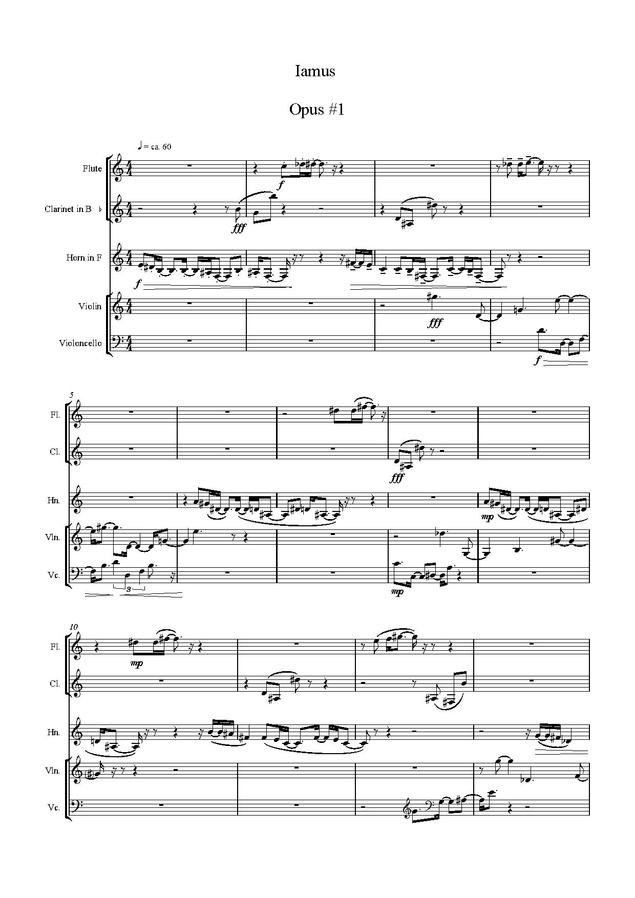
\includegraphics[width=0.4\linewidth]{rys01/lamus_notes.jpg}
    \caption{
      Zapis nutowy utworu \textit{Opus One},
      wygenerowany przez komputer \textit{Lamus}.
    }\label{fig:lamus_notes}
\end{figure}

Druga grupa algorytmów, generująca pliki audio, bazuje na klasie algorytmów
wywodzących się ze \textit{Stable Diffusion}~\cite{stablediffusion}.
Modele generujące pliki audio zgodne z opisem tekstowym 
(przykładowo \texttt{,,smutny jazz''} bądź \texttt{,,muzyka taneczna w stylu Depeche Mode''})
szkolone są w taki sam sposób jak algorytmy \textit{stable diffusion},
dane treningowe składają się z obrazów spektrogramów~\cite{riffusion}. 
Po trenowaniu, model jest wstanie wygenerować spektrogram zawierający
utwór muzyczny zgodny z poleceniem użytkownika (\ref{fig:riffusion_spectro}).
Wygenerowany przez model spektrogram jest konwertowany 
do sygnału dżwiękowego za pomocą odwrotnej transformaty Fouriera.

\begin{figure}[H]
    \centering
    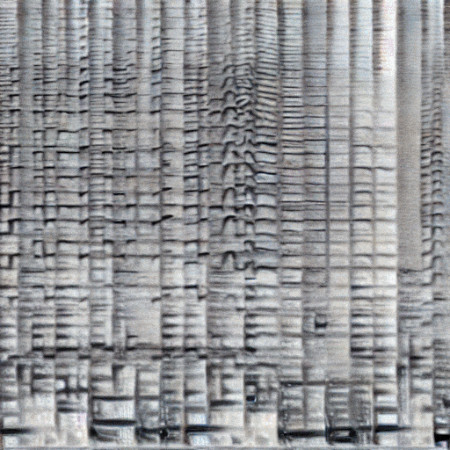
\includegraphics[width=0.4\linewidth]{rys01/riffusion_spectro.jpg}
    \caption{
      Przykładowy spektrogram wygenerowany przez algorytm \textit{Stable Riffusion}
      dla danych wejściowych \texttt{funk bassline with a jazzy saxophone solo}.
    }\label{fig:riffusion_spectro}
\end{figure}

Trzecia grupa algorytmów, symulowanie brzemienia instrumentów muzycznych, najczęściej wykorzystuje sieci
neuronowe trenowane na brzmieniu prawdziwych instrumentów~\cite{engel2017neural}~\cite{engel2020ddsp}. 
Tego typu algorytmy pozwalają symulowanie instrumentów o złożonych barwach, takich jak instrumenty
smyczkowe lub dęte oraz na płynne przechodzenie między brzmieniami różnych instrumentów muzycznych.

% TODO: check later
% https://github.com/Kinyugo/msanii

Metody opisane w rozdziale~\ref{traditional_algos} można porównać pod względem ich przydatności
dla użytkownika końcowego, czyli osoby zajmującej się produkcją nagrań muzycznych. Metoda pierwsza, 
generowanie zapisu symbolicznego, może wydawać się mniej zaawansowana niż generowanie całych plików dźwiękowych.
Jednakże, z perspektywy użytkownika, zapis symboliczny jest bardziej praktyczny,
ponieważ możliwe jest zaimportowanie go do programu DAW i późniejsza modyfikacja zapisu nutowego.
Obecnie dostępne modele generujące pełne nagrania z muzyką nie umożliwiają
szczegółowego edytowania parametrów wygenerowanego dźwięku, ponieważ operują bardzo wysokopoziomowo 
-- syntezują muzykę na podstawie opisu słownego. Podobne problemy występują również podczas wykorzystywania
algorytmów z grupy trzeciej, głębokie sieci neuronowe nie są przystosowane do ręcznej modyfikacji przez użytkownika.

Podsumowując, wykorzystanie wygenerowanego przez komputer zapisu nutowego jest proste,
ze względu na symboliczną naturę zapisu.
Wykorzystanie wygenerowanego przez komputer dźwięku jest ograniczone ze względu na fakt,
że do generowania złożonych sygnałów dźwiękowych wykorzystywane są techniki takie jak
głębokie sieci neuronowe, w których utrudniona jest dokładna kontrola nad konkretnymi
parametrami funkcjonowania sieci.

Niniejsza praca sugeruje nową metodę podejścia do problemu generowania sygnałów dźwiękowych,
którego nie da się zaklasyfikować do żadnej z wyżej wymienionych~(\ref{traditional_algos}) dziedzin komputerowej kompozycji muzycznej.
Graf przetwarzania sygnałów wytworzony przez algorytm implementowany w ramach pracy magisterskiej jest przepisem na gotowy elektroniczny instrument muzyczny,
który może być wykorzystany w programie do komponowania muzyki. Algorytm nie generuje bezpośrednio sygnału dźwiękowego, lecz tworzy
graf przetwarzania sygnałów, który jest zrozumiały dla użytkownika i pozwala na precyzyjne dostosowanie parametrów syntezy.
Tego typu proces generowania grafów przetwarzania sygnałów dźwiękowych może być porównany z procesem projektowania instrumentu muzycznego.

Modyfikowanie ścieżki przetwarzania sygnału jest techniką często wykorzystywaną w muzyce
elektronicznej, do tworzenia dźwięków o interesującej barwie bądź dynamice. Syntezatory dźwięku
dostępne na rynku często wyposażone są w tzw. \textit{patch bay}~(\ref{fig:mother32}), pozwalający na modyfikowanie
grafu przepływu sygnałów wewnątrz syntezatora, bądź połączenie go z zewnętrznym sprzętem muzycznym
bądź elektronicznym.

\begin{figure}[H]
    \centering
    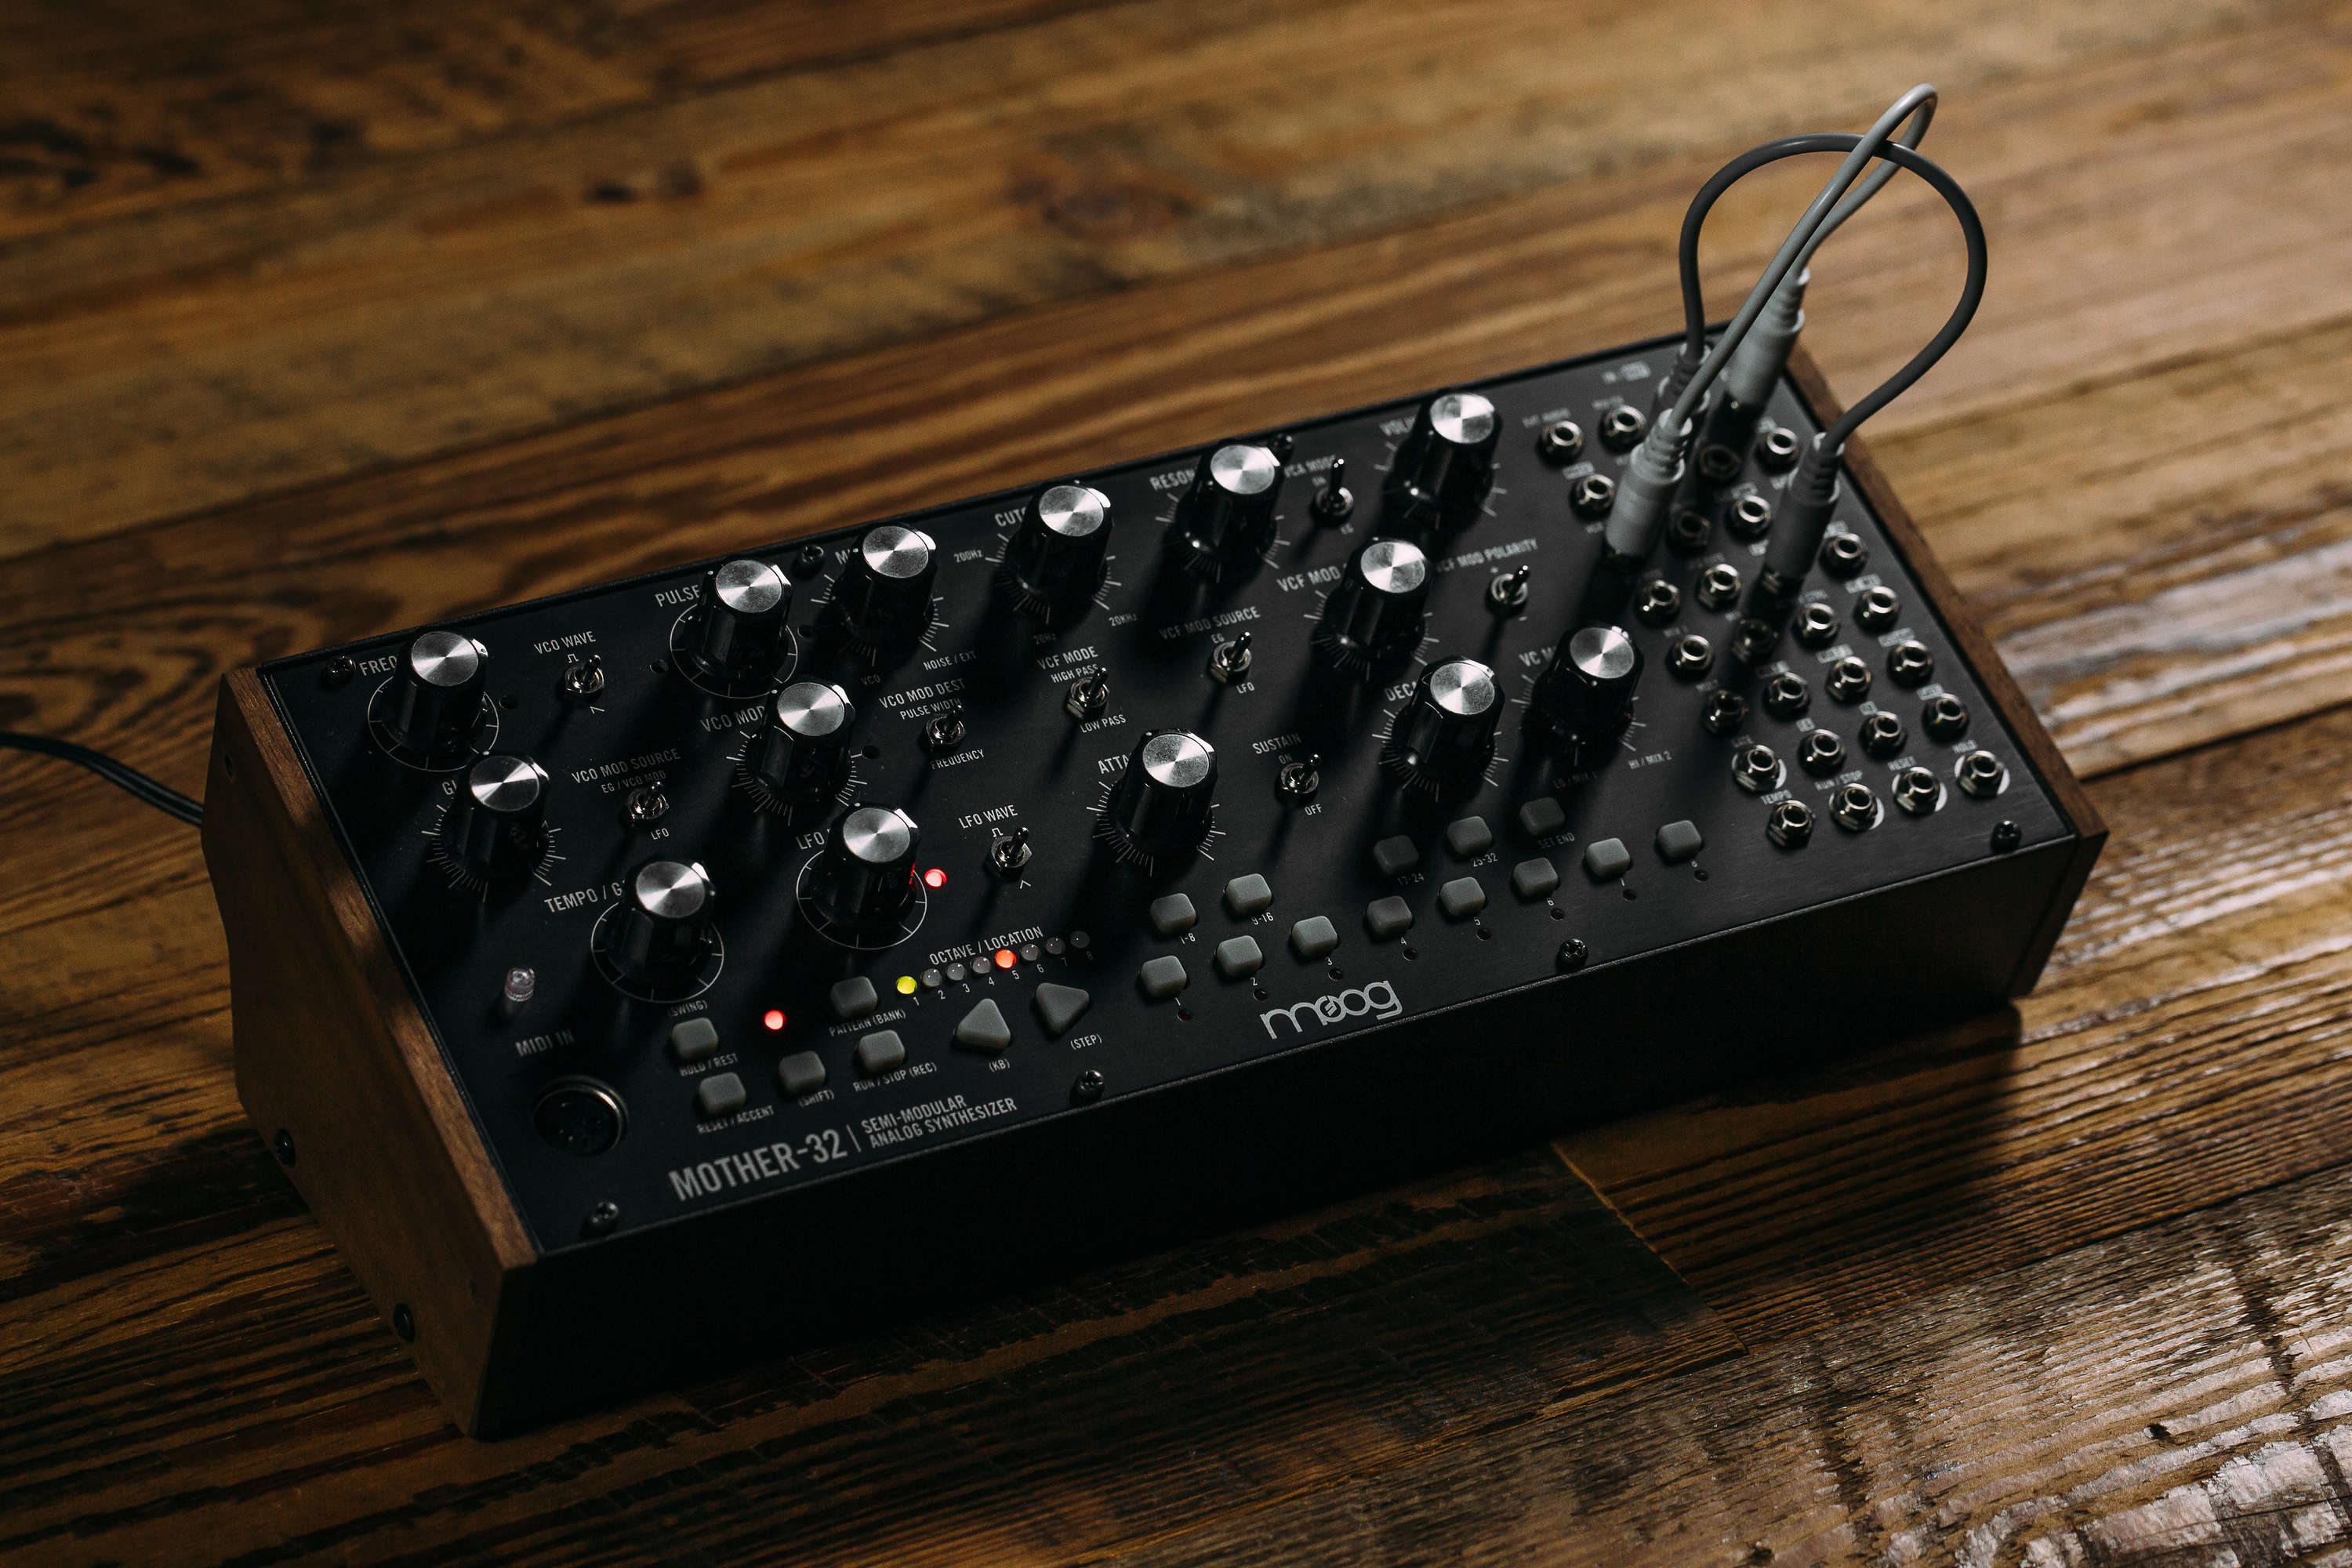
\includegraphics[width=0.7\linewidth]{rys01/mother32.jpg}
    \caption{
      Syntezator \textit{Mother 32} firmy \textit{Moog}, po prawej stronie widoczny
      jest \textit{patch bay} z podłączonymi przewodami, które nadpisują konfigurację
      połączeń między układami generującymi i przetwarzającymi sygnał dźwiękowy.
    }\label{fig:mother32}
\end{figure}


\section{Cel pracy}

Celem pracy jest \textbf{opracowanie algorytmu generacji grafów przetwarzania sygnałów, który
który wykona syntezę próbki dźwięku zadanej przez użytkownika}.
Problem poruszany w pracy można zakwalifikować do grupy zagadnień związanych
z pojęciami \textit{computer-aided design} oraz \textit{generative artificial intelligence}, zastosowanymi w dziedzienie inżynierii dźwięku. Docelowo
zaimplementowany algorytm będzie automatyzował pracę inżyniera dźwięku,
tworząc i konfigurując grafy przetwarzania sygnałów dźwiękowych, dostępne w
programach typu \textit{digital audio workstation}~(\ref{fig:ableton_patch}). Badania obejmują dwa zagadnienia:
\textbf{
\begin{enumerate}\label{research_types}
    \item opracowanie metody generowania grafu przetwarzania sygnałów oraz późniejszej modyfikacji grafu -- jego struktury i parametrów,
    \item dobór funkcji celu, na podstawie której algorytm optymalizujący będzie modyfikował graf przetwarzania sygnałów.
    \item przeprowadzenie badań symulacyjnych, które zweryfikują skuteczność opracowanego algorytmu.
    \item porównanie wyników badań symulacyjnych z pracami naukowymi o podobnej tematyce.
\end{enumerate}
}

\begin{figure}[H]
    \centering
    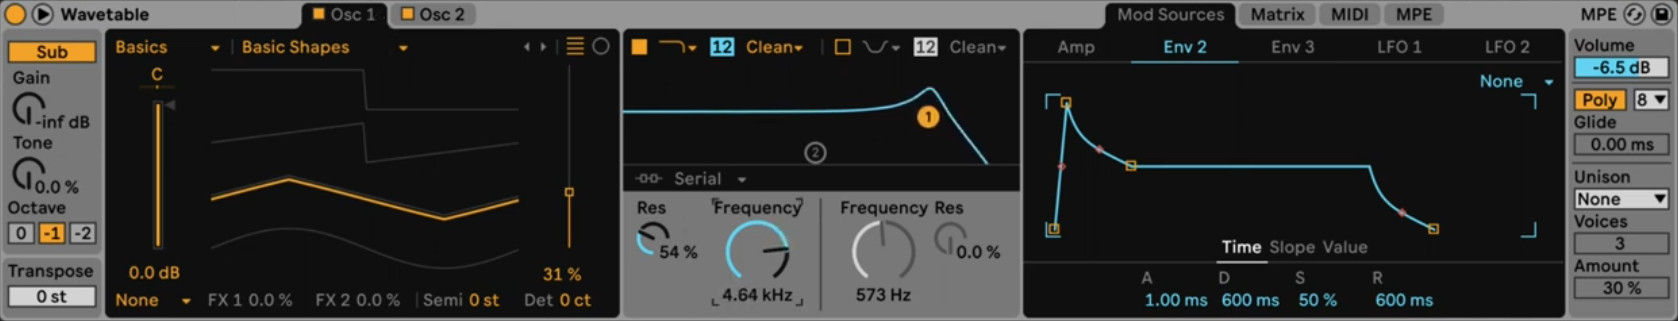
\includegraphics[width=0.8\linewidth]{rys01/ableton_patch.jpg}
    \caption{
      Zbiór parametrów konfigurujących syntezator dźwięku \textit{Wavetable} w programie \textit{Ableton}
    }\label{fig:ableton_patch}
\end{figure}

\subsection{Podstawy syntezy dźwięku}\label{sec:basics_of_sound_synthesis}

W syntezie dźwięku wykorzystuje się algorytmy generujące
i przetwarzające sygnały w zakresie częstotliwości słyszalnych.
Praca wykorzystuje powszechnie używane typy algorytmów syntezy,
opisane w~\cite{computational_music_synthesis}.

\subsubsection{Synteza FM}

Synteza FM wykorzystuje sygnał sinusoidalny jako źródło sygnału podstawowego
(\textit{carrier}). Zróżnicowane barwy dźwięku uzyskiwane są przez modulowanie
częstotliwości sinusoidy podstawowej przez inne sygnały sinusoidalne (\textit{modulators}),
które zazwyczaj generują sygnał o częstotliwości będącej wielokrotnością
częstotliwości podstawowej~\cite{spectral_audio_processing}. Siła modulacji
może być zmieniana w trakcie syntezy, co powoduje zmiany
w odczuwanej barwie dźwięku.

\subsubsection{Synteza subtraktywna}

W syntezie subtraktywnej wykorzystuje się sygnały dźwiękowe o dużej liczbie
składowych harmonicznych, takie jak sygnał piłokształtny lub kwadratowy.
Podstawową barwę dźwięku uzyskuje się przez dobór kilku sygnałów
o różnych kształtach, następnie sygnał jest filtrowany za pomocą filtrów
dolno-, górno- i pasmoprzepusowych~\cite{digital_filters}, aby
usunąć wybrane przez użytkownika składowe częstotliwościowe.
Dynamiczne zmiany w barwie dźwięku uzyskuje się poprzez modulowanie
częstotliwości odcięcia filtru.

\subsubsection{Algorytmy \textit{physical modeling}}

Algorytmy typu \textit{physical modeling} wykorzystują uproszczone
modele fizyczne rzeczywistych obiektów wytwarzających sygnały dźwiękowe,
takie jak struny czy membrany~\cite{lisp_synthesis}.


\subsubsection{symulacja efektu pogłosu/echa~\cite{reverb}~\cite{freeverb}}

Sygnał wygenerowany przez dany algorytm syntezy (lub połączenie wielu algorytmów)
może być przetworzony przez algorytmy symulujące echo lub pogłos (\textit{reverb, delay}).
Tego typu algorytmy naśladują roznoszenie się dźwięku w pudle rezonansowym
instrumentu bądź w dużej przestrzeni (sala koncertowa, jaskinia).
 

\subsection{Generowanie grafu przetwarzania sygnałów}

Proces syntezy dźwięku często jest przedstawiany jako graf przetwarzania sygnałów, w którym
każdy węzeł wykonuje na sygnale określoną operację.
Przykładowy graf przetwarzania sygnału dla syntezatora analogowego subtraktywnego
przedstawiony jest na schemacie~\ref{fig:minilogue_diagram}.
Pierwsze zagadnienie poruszane w pracy sprowadza się do opracowania algorytmu pozwalającego na wygenerowanie
grafu przetwarzania sygnałów DSP oraz jego późniejszą modyfikację. Przykładem modyfikacji grafu
może być wprowadzanie do niego nowych źródeł modulacji bądź zmiana algorytmu generującego sygnał.

\begin{figure}[H]
    \centering
    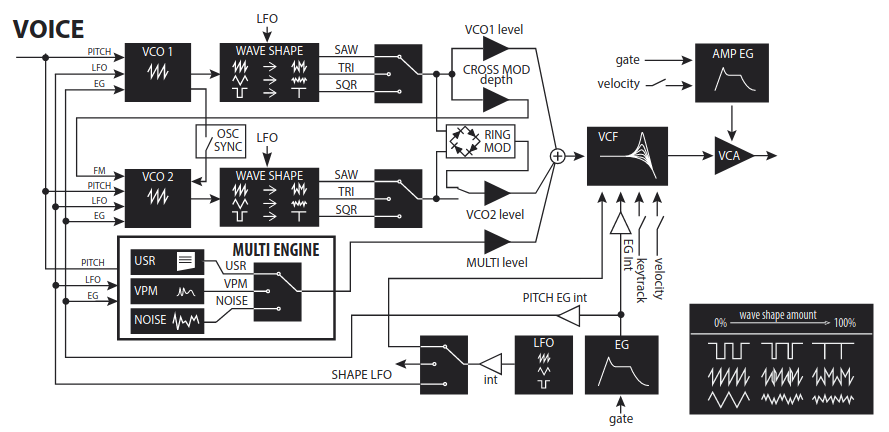
\includegraphics[width=0.8\linewidth]{rys01/minilogue_voice_block_diagram.png}
    \caption{
      Diagram blokowy pojedynczego głosu w syntezatorze 
      \textit{Minilogue xd} firmy \textit{Korg}~\cite{minilogue_diagram}.
    }\label{fig:minilogue_diagram}
\end{figure}

\subsection{Funkcja celu oceniająca podobieństwo barwy dźwieku}

Drugie zagadnienie obejmuje przetestowanie szeregu algorytmów, które można
wykorzystać do zbudowania funkcji celu, która będzie optymalizowana
poprzez~,,dostrajanie'' parametrów i struktury grafu przetwarzania sygnałów dźwiękowych.
Problem porównywania barwy dwóch sygnałów dźwiękowych nie jest problemem trywialnym,
ponieważ wymaga zamodelowania wrażeń psychoakustycznych~\cite{engel2020ddsp} odczuwanych
podczas odsługu próbki dźwięku.
Skuteczność danej funkcji celu finalnie musi być poddana subiektywnej ocenie,
ponieważ nie istnieją obiektywne metryki mierzące z natury subiektywne odczucia słuchacza.
Praca proponuje wykorzystanie współczynników cepstralnych sygnału (MFCC) w połączeniu
z dynamicznym skalowaniem czasu (\textit{dynamic time wrapping}, DTW) jako funkcji celu.
Proces wyboru funkcji celu został
opisany w rozdziale~\ref{target_function_chapter}.

\subsection{Problem optymalizacyjny}

W pracy rozwiązywany jest problem optymalizacyjny, w którym
struktura oraz parametry grafu przetwarzania sygnałów dostosowywane
są tak, aby wygenerować zadaną próbkę dźwięku. Tak wytworzony
graf może być wykorzystany jako elektroniczny instrument muzyczny. 

% Następnie, dla danego układu $N$ węzłów przetwarzania oraz dla macierzy połączeń $C$, 
% należy rozwiązać następujący problem optymalizacji, należy rozwiązać problem
% maksymalizacji funkcji opisanej równaniem~\ref{eq:target_function} dla
% parametrów wszystkich wejść $i_j$ oraz $o_j$, które nie są połączone bezpośrednio
% pomiędzy węzłami.




\section{Zakres pracy, plan badań}\label{chap:thesis_scope}

\subsection{Metody generowania grafu przetwarzania sygnałów oraz późniejsza modyfikacja grafu}

Głównym problemem przy generowaniu grafu przetwarzania sygnałów są ograniczenia nałożone na strukturę grafu,
które należy spełnić, by graf był logicznie interpretowalny jako łańcuch przetwarzania sygnałów.
Graf musi być grafem skierowanym, który nie zawiera pętli o dodatnim sprzężeniu zwrotnym.
% Struktura grafu powinna być możliwie jak najbardziej przejrzysta dla użytkownika. 
Automatyczna ewolucja może dążyć w kierunku wykorzystania nadmiarowej liczby
bloków przetwarzania sygnału, jeśli funkcja celu nie będzie zawierała kary za zbyt złożone grafy.
Podobne prace~\cite{evolutionary_puredata} wykorzystują podejście oparte o 
\textit{mixed-typed carthesian genetic programming}, które będzie punktem startowym dla pracy.
Finalnie, badania dążą do wyznaczenia algorytmu o następujący właściwościach:

\begin{enumerate}
    \item algorytm generuje grafy będące logicznie spójnymi łańcuchami przetwarzania dźwięku (skierowany, bez pętli o dodatnim sprzężeniu zwrotnym w natężeniu sygnału),
    \item algorytm maksymalizuje wykorzystanie poszczególnych bloków przetwarzania w grafie, co minimalizuje finalny rozmiar grafu, czyniąc go bardziej czytelnym,
    \item generowany graf posiada reprezentację umożliwiającą wykonanie krzyżowania dwóch grafów przetwarzania sygnału. Graf będący wynikiem krzyżowania nadal musi być poprawnym grafem przetwarzania sygnału.
\end{enumerate}

\noindent
Elementami grafu przetwarzania sygnałów są używane powszechnie w syntezie dźwięku algorytmy,
opisane w sekcji~\ref{sec:basics_of_sound_synthesis}.

\subsection{Dobór funkcji błędu: różnica między wygenerowanym a docelowym sygnałem dźwiękowym}

Funkcja celu poszukiwana w ramach projektu musi określać, jak dobrze sygnał wygenerowany przez
graf przetwarzania sygnałów pokrywa się z sygnałem docelowym. Porówanie sygnałów musi skupiać się
na cechach sygnału, które są najbardziej słyszalne dla ludzkiego ucha. Jednocześnie funkcja nie powinna
,,karać'' sygnałów, które są względem siebie przesunięte w fazie. Wśród algorytmów, które zostały wybrane
do przetestowania w ramach projektów zawarte są:

\begin{enumerate}
  \item algorytmy porównywania sygnałów oparte o transformatę Fouriera~\cite{sliding_fourier}~\cite{mfcc},
  \item techniki wykorzystywane do generowania~,,cyfrowych podpisów'' sygnałów dźwiękowych (\textit{sound fingerprinting})~\cite{computer_vision_music_identification},
  \item algorytmy wykrywające spadek jakości dźwięku z perspektywy psychoakustycznej~\cite{peaq}~\cite{frechet_audio_distance}.
\end{enumerate}

\section{Struktura i zawartość pracy}

% Praca podzielona jest na następujące części:

Rozdział \textbf{Definicja problemu} formalizuje i opisuje problem optymalizacyjny rozwiązywany w pracy.
W rozdziale \textbf{Analiza i wybór funkcji celu} opisano proces porównywania funkcji z dziedziny przetwarzania sygnałów,
które pozwalają określić jak podobna jest barwa dźwięku dwóch sygnałów dźwiękowych i
uzasadniono wybór funkcji celu, która została zastosowana w pracy.
Rozdział \textbf{Algorytm rozwiązania} opisuje algorytm wykorzystany do rozwiązania problemu
zdefiniowanego w rozdziale~\ref{chap:problem_definition}.
W rozdziale \textbf{Implementacja grafu przetwarzania sygnałów} opisane zostało zaimplementowane w ramach pracy środowisko eksperymentalne,
pozwalające na wytwarzanie grafów przetwarzania sygnałów o dowolnej strukturze.
Przedstawione są w nim również zaimplementowane algorytmy syntezy i przetwarzania sygnałów dźwiękowych.
Rozdział \textbf{Badania symulacyjne} opisuje proces badawczy, w którym narzędzia wytworzone w
rozdziałach~\ref{dsp_graph_chapter} oraz~\ref{target_function_chapter}
zostały wykorzystane do automatycznego wytworzenia grafu DSP, który naśladuje barwę zadanej próbki dźwięku.
Porównuje uzyskane wyniki z podobną pracą badawczą~\cite{evolutionary_puredata}.
Rozdział \textbf{Analiza wyników, możliwe drogi dalszego rozwoju} podsumowuje uzyskane wyniki badań, podejmuje dyskusję nad ogólną skutecznością i przydatnością zaimplementowanego rozwiązania oraz
kreśli potencjalne drogi dalszego rozwoju prac badawczych w podobnej tematyce. W czasie, gdy niniejsza praca była tworzona, zostały opublikowane badania
dotyczące podobnego problemu~\cite{ieee_synth_programming}, rozdział podejmuje dyskusję o różnicach w podejściu do problemu oraz potencjalnych
zalet i wad każdego z podejść. \textbf{Dodatek A} zawiera instrukcję wdrożeniową dla
zaimplementowanego w ramach pracy środowiska eksperymentalnego, w \textbf{Dodatku B}
opisana jest zawartość załączonej do pracy płyty DVD\@.

+). Druga, jeśli zostanie zastosowana, pozwala określić, które z~plików zostaną skompilowane w całości (na przykład kod źródłowy pierwszego i drugiego rozdziału \verb+\includeonly{rozdzial01.tex,rozdzial02.tex}+). Brak nazwy pliku na liście w poleceniu \verb+\includeonly+ przy jednoczesnym wystąpieniu jego nazwy w poleceniu \verb+\include+ oznacza, że w kompilacji zostaną uwzględnione referencje wygenerowane dla tego pliku wcześniej, sam zaś kod źródłowy pliku nie będzie kompilowany. 

% W szablonie wykorzystano klasę dokumentu \texttt{memoir} oraz wybrane pakiety. Podczas kompilacji szablonu w \texttt{MikTeXu} wszelkie potrzebne pakiety zostaną zainstalowane automatycznie (jeśli \texttt{MikTeX} zainstalowano z opcją dynamicznej instalacji brakujących pakietów). W przypadku innych dystrybucji \LaTeX-a może okazać się, że pakiety te trzeba doinstalować ręcznie (np.\ pod linuxem z \texttt{TeXLive} trzeba doinstalować dodatkową zbiorczą paczkę, a jeśli ma się menadżera pakietów \LaTeX-owych, to pakiety te można instalować indywidualnie).

% Jeśli w szablonie będzie wykorzystany indeks rzeczowy, kompilację źródeł trzeba będzie rozszerzyć o kroki potrzebne na wygenerowanie plików pośrednich \texttt{Dokument.idx} oraz \texttt{Dokument.ind} oraz dołączenia ich do finalnego dokumentu (podobnie jak to ma miejsce przy generowaniu wykazu literatury).
% Szczegóły dotyczące generowania indeksu rzeczowego opisano w podrozdziale~\ref{sec:indeks}.

% \section{Sprawdzanie poprawności tekstu}
% Większość środowisk ułatwiających pisanie \LaTeX-owych dokumentów wspiera sprawdzenie poprawności tekstu (ang.~\emph{spell checking}). Wystarczy odpowiednio je skonfigurować. Niestety, proponowana przez narzędzia korekta nie jest genialna. Bazuje ona na prostym porównywaniu wyrazów (z końcówkami). Nie wbudowano w nią żadnej większej inteligencji. Tak więc proszę nie porównywać jej z korektą oferowaną w narzędziach MS Office (tam jest ona dużo bardziej zaawansowana).

% \texttt{TeXnicCenter} korzysta ze słowników do pobrania ze strony \texttt{openoffice} (\url{https://extensions.openoffice.org/}).
% Aby sprawę uprościć słowniki dla języka polskiego (pliki \texttt{pl\_PL.aff} oraz \texttt{pl\_PL.dic}) dołączono do szablonu (są w katalogu \texttt{Dictionaries}). Pliki te należy umieścić w katalogu \texttt{C:\textbackslash{}Program Files\textbackslash{}TeXnicCenter\textbackslash{}Dictionaries}, a w konfiguracji projektu (\texttt{Tools/Options/Spelling}) należy wybrać \texttt{Language: pl}, \texttt{Dialect: PL}. Jeśli główny tekst pracy pisany jest w innym języku, to trzeba zmienić słownik.

% Zaskakujące może jest to, że \emph{spell checker} w \texttt{TeXnicCenter} działa zarówno przy pracy na plikach UTF8, jak i na plikach ANSI. Jeśli byłyby jakieś problemy ze słownikiem wynikające z~kodowania znaków, wtedy słownik trzeba przekodować. To powinno pomóc.

% \section{Wersjonowanie}
% W trakcie edytowania pracy w systemie latex dobrą praktyką jest wersjonowanie tworzonego kodu. Do wersjonowania zaleca się wykorzystać system \texttt{git}. Opis sposobu pracy z tym systemem opisano w licznych tutorialach dostępnych w sieci. Szczególnie godnym polecenia zasobem jest strona domowa projektu \url{https://git-scm.com/}.

% Zwykle pracę z systemem wersjonowania rozpoczyna się od utworzenia repozytorium zdalnego i lokalnego. Lokalne służy do bieżącej pracy, zdalne -- do współpracy z innymi użytkownikami (z promotorem). 

% Po utworzeniu repozytorium lokalnego i roboczej gałęzi (czy będzie to \texttt{master} czy inna gałąź -- ustalają to sami zainteresowani) należy skopiować do niego wszystkie pliki dostarczone w szablonie, a po ich wstępnym przeredagowaniu należy je zaznaczyć do wersjonowania. Potem należy wysłać zmiany na repozytorium zdalne (możliwa jest też ścieżka odwrotna, można zacząć od zmian na repozytorium zdalnym, które pobrane będą do repozytorium lokalnego).

% Podczas kompilowania projektu będą powstawały pliki pomocnicze. Plików tych nie należy wersjonować (zabierają niepotrzebnie miejsce, a przecież zawsze można je odtworzyć uruchamiając kompilację na źródłach). \texttt{git} posiada mechanizm automatycznego odrzucania plików niepodlegających wersjonowaniu. Mechanizm ten bazuje na wykorzystaniu pliku konfiguracyjnego \texttt{.gitignore} zamieszczonego w katalogu głównym repozytorium. O szczegółach \texttt{.gitignore} można poczytać  na stronie \url{https://git-scm.com/docs/gitignore}. 

% W sieci można znaleźć liczne propozycje plików konfiguracyjnych \texttt{.gitignore} dopasowanych do potrzeb latexowej kompilacji. Nie trzeba ich jednak szukać. W~szablonie zamieszczono przykładowy taki plik. Zawiera on, między innymi, wpis zabraniający wersjonowania pliku wynikowego \texttt{Dyplom.pdf}. 


% Plik \texttt{.gitignore} należy umieścić w repozytorium zaraz po jego utworzeniu. Jeśli w repozytorium pojawiły się już jakieś zmiany zanim pojawił się tam \texttt{.gitignore}, to wtedy należy wykonać kroki opisane na stronie: \url{https://stackoverflow.com/questions/38450276/force-git-to-update-gitignore/38451183}

% \begin{lstlisting}[basicstyle=\small\ttfamily]
% > > > > You will have to clear the existing git cache first.
%     git rm -r --cached .
% > > > > Once you clear the existing cache, adds/stages all of the files in the current directory and commit
%     git add .
%     git commit -m "Suitable Message"
% > > > > 
% \end{lstlisting}


% Zalecany schemat współpracy dyplomanta z promotorem polega na wykonywaniu w kolejnych iteracjach następujących kroków:
% \begin{itemize}
% \item dyplomant edytuje wybraną część pracy, a po skończeniu edycji wrzuca zmiany do zdalnego repozytorium,
% \item dyplomant informuje promotora o zakończeniu etapu prac,
% \item dyplomant może zacząć edycję kolejnego fragmentu pracy, a w tym czasie promotor może dokonać oceny/korekty zmian pobranych ze zdalnego repozytorium,
% \item promotor wrzuca dokonane przez siebie zmiany do zdalnego repozytorium, informując o tym dyplomanta.
% \end{itemize}
% Główna zasada tego schematu polega na niedoprowadzaniu do konfliktów (nadpisywania zmian). Jeśli jednak takie konflikty nastąpią, można je niwelować poprzez odpowiednie scalanie zmian (merdżowanie). Swoją drogą, niezłym narzędziem do porównywania zawartości plików i~usuwania niezgodności jest \texttt{WinMerge} (\url{https://winmerge.org/}).


% Do wzajemnych powiadomień można wykorzystać pocztę elektroniczną. Można też spróbować wdrożyć mechanizm zatwierdzania zmian (ang.~\emph{merge requests}). Można też umówić się na sprawdzanie zawartości repozytorium zgodnie z jakimś przyjętym harmonogramem. Ważne, by wiadomo było obu stronom, na jakim schemacie współpracy mają bazować.

% Dobrą praktyką jest też wstawianie w kod komentarzy. Przyjętą powszechnie konwencją jest rozpoczynanie komentarzy od:
% \begin{itemize}
% \item \verb|% TO DO: tekst zalecenia| 
% -- jeśli jest to jakieś zalecenie promotora, czy też 
% \item \verb|% DONE: tekst wyjaśnienia| 
% -- jeśli jakieś zalecenie zostało wykonane przez dyplomanta. 
% \end{itemize}

% Jako zdalne repozytorium można wykorzystać: \texttt{github}, \texttt{bitbucket}, \texttt{gitlab} (są to serwisy, które pozwalają zarządzać repozytoriami \texttt{git}).
% Dobrą praktyką jest też uruchomienie klientów git oferujących graficzny interfejs (jak \texttt{SourceTree}, \texttt{GitCracken} itp.). W narzędziach tych można zobaczyć natychmiast na czym polegały wprowadzone w repozytorium zmiany. 
